\begin{titlepage}
    \begin{tikzpicture}[remember picture,overlay,inner sep=0,outer sep=0]
        % Outer frame
        \draw[blue!70!black,line width=4pt]
        ([xshift=-2cm,yshift=-2cm]current page.north east) coordinate (A) --
        ([xshift=2cm,yshift=-2cm]current page.north west) coordinate (B) --
        ([xshift=2cm,yshift=2cm]current page.south west) coordinate (C) --
        ([xshift=-2cm,yshift=2cm]current page.south east) coordinate (D) -- cycle;

        % First decorative inner line
        \draw
        ([yshift=0.5cm,xshift=-0.5cm]A) --
        ([yshift=0.5cm,xshift=0.5cm]B) --
        ([yshift=-0.5cm,xshift=0.5cm]B) --
        ([yshift=-0.5cm,xshift=-0.5cm]B) --
        ([yshift=0.5cm,xshift=-0.5cm]C) --
        ([yshift=0.5cm,xshift=0.5cm]C) --
        ([yshift=-0.5cm,xshift=0.5cm]C) --
        ([yshift=-0.5cm,xshift=-0.5cm]D) --
        ([yshift=0.5cm,xshift=-0.5cm]D) --
        ([yshift=0.5cm,xshift=0.5cm]D) --
        ([yshift=-0.5cm,xshift=0.5cm]A) --
        ([yshift=-0.5cm,xshift=-0.5cm]A) --
        ([yshift=0.5cm,xshift=-0.5cm]A);

        % Second decorative inner line
        \draw
        ([yshift=-0.3cm,xshift=0.3cm]A) --
        ([yshift=-0.3cm,xshift=-0.3cm]B) --
        ([yshift=0.3cm,xshift=-0.3cm]B) --
        ([yshift=0.3cm,xshift=0.3cm]B) --
        ([yshift=-0.3cm,xshift=0.3cm]C) --
        ([yshift=-0.3cm,xshift=-0.3cm]C) --
        ([yshift=0.3cm,xshift=-0.3cm]C) --
        ([yshift=0.3cm,xshift=0.3cm]D) --
        ([yshift=-0.3cm,xshift=0.3cm]D) --
        ([yshift=-0.3cm,xshift=-0.3cm]D) --
        ([yshift=0.3cm,xshift=-0.3cm]A) --
        ([yshift=0.3cm,xshift=0.3cm]A) --
        ([yshift=-0.3cm,xshift=0.3cm]A);
    \end{tikzpicture}

    \begin{center}
        \vspace{-0.7cm}
        \textbf{\large TRƯỜNG ĐẠI HỌC BÁCH KHOA} \\
        \textbf{\large ĐẠI HỌC QUỐC GIA THÀNH PHỐ HỒ CHÍ MINH} \\
        \textbf{\large KHOA KHOA HỌC VÀ KỸ THUẬT MÁY TÍNH}\\
        
\includegraphics[scale=0.5]{./cover_pages/decor_char.png}
    \end{center}

    \vspace{0.5cm}

    \begin{figure}[h!]
        \begin{center}
            
\includegraphics[height=5cm]{cover_pages/01_logobachkhoasang.png}
        \end{center}
    \end{figure}
    \vspace{1cm}
    \begin{center}
        {\fontsize{18pt}{24pt}\selectfont \textbf{BÁO CÁO BÀI TẬP LỚN}}\\
        {\fontsize{18pt}{24pt}\selectfont \textbf{MÔN HỌC: ĐẠI SỐ TUYẾN TÍNH}}\\
    \end{center}
    \begin{center}
        \vspace{0.5cm}
        {\fontsize{18pt}{24pt}\selectfont \textbf{\textit{ĐỀ TÀI 8}:}}\\
        \vspace{0.3cm}
        \textbf{{\fontsize{18pt}{24pt}\selectfont Thuật toán Floyd - Warshall \\ tìm đường đi ngắn nhất
                }}\\
        \vspace{0.5cm}
    \end{center}

    \hspace{2cm}
    \begin{minipage}{0.8\textwidth} % Instead of \textwidth
        \vspace{0.5cm}
        \begin{tabular}{ll}
            {\fontsize{16pt}{24pt}\selectfont \textbf{GVHD:}} & {\fontsize{16pt}{24pt}\selectfont \textbf{Th.S Nguyễn Xuân Mỹ}} \\
            {\fontsize{16pt}{24pt}\selectfont \textbf{Lớp:}}  & {\fontsize{16pt}{24pt}\selectfont \textbf{L15}}                 \\
            {\fontsize{16pt}{24pt}\selectfont \textbf{Nhóm:}} & {\fontsize{16pt}{24pt}\selectfont \textbf{8}}                   \\
        \end{tabular}
    \end{minipage}


    \vspace{2.7cm}
    \centerline{\Large TP. Hồ Chí Minh, 5/2025}
\end{titlepage}
